\documentclass{book}
\usepackage[a4paper,top=2.5cm,bottom=2.5cm,left=2.5cm,right=2.5cm]{geometry}
\usepackage{makeidx}
\usepackage{natbib}
\usepackage{graphicx}
\usepackage{multicol}
\usepackage{float}
\usepackage{listings}
\usepackage{color}
\usepackage{ifthen}
\usepackage[table]{xcolor}
\usepackage{textcomp}
\usepackage{alltt}
\usepackage{ifpdf}
\ifpdf
\usepackage[pdftex,
            pagebackref=true,
            colorlinks=true,
            linkcolor=blue,
            unicode
           ]{hyperref}
\else
\usepackage[ps2pdf,
            pagebackref=true,
            colorlinks=true,
            linkcolor=blue,
            unicode
           ]{hyperref}
\usepackage{pspicture}
\fi
\usepackage[utf8]{inputenc}
\usepackage{mathptmx}
\usepackage[scaled=.90]{helvet}
\usepackage{courier}
\usepackage{sectsty}
\usepackage[titles]{tocloft}
\usepackage{doxygen}
\lstset{language=C++,inputencoding=utf8,basicstyle=\footnotesize,breaklines=true,breakatwhitespace=true,tabsize=8,numbers=left }
\makeindex
\setcounter{tocdepth}{3}
\renewcommand{\footrulewidth}{0.4pt}
\renewcommand{\familydefault}{\sfdefault}
\hfuzz=15pt
\setlength{\emergencystretch}{15pt}
\hbadness=750
\tolerance=750
\begin{document}
\hypersetup{pageanchor=false,citecolor=blue}
\begin{titlepage}
\vspace*{7cm}
\begin{center}
{\Large J\-S\-O\-N-\/\-D\-P\-Final }\\
\vspace*{1cm}
{\large Generated by Doxygen 1.8.0}\\
\vspace*{0.5cm}
{\small Mon Jun 25 2012 05:36:36}\\
\end{center}
\end{titlepage}
\clearemptydoublepage
\pagenumbering{roman}
\tableofcontents
\clearemptydoublepage
\pagenumbering{arabic}
\hypersetup{pageanchor=true,citecolor=blue}
\chapter{Class Index}
\section{Class Hierarchy}
This inheritance list is sorted roughly, but not completely, alphabetically\-:\begin{DoxyCompactList}
\item \contentsline{section}{\-\_\-bj}{\pageref{struct__bj}}{}
\item \contentsline{section}{Json\-Builder}{\pageref{class_json_builder}}{}
\begin{DoxyCompactList}
\item \contentsline{section}{Concrete\-Builder}{\pageref{class_concrete_builder}}{}
\end{DoxyCompactList}
\item \contentsline{section}{Json\-Exception}{\pageref{class_json_exception}}{}
\begin{DoxyCompactList}
\item \contentsline{section}{Data\-Not\-Found\-Exception}{\pageref{class_data_not_found_exception}}{}
\item \contentsline{section}{Incorrect\-Json\-Exception}{\pageref{class_incorrect_json_exception}}{}
\item \contentsline{section}{Not\-Json\-Array\-Exception}{\pageref{class_not_json_array_exception}}{}
\item \contentsline{section}{Not\-Json\-Object\-Exception}{\pageref{class_not_json_object_exception}}{}
\end{DoxyCompactList}
\item \contentsline{section}{Json\-Value}{\pageref{class_json_value}}{}
\begin{DoxyCompactList}
\item \contentsline{section}{Json\-Array}{\pageref{class_json_array}}{}
\item \contentsline{section}{Json\-Boolean}{\pageref{class_json_boolean}}{}
\item \contentsline{section}{Json\-Double}{\pageref{class_json_double}}{}
\item \contentsline{section}{Json\-Null}{\pageref{class_json_null}}{}
\item \contentsline{section}{Json\-Object}{\pageref{class_json_object}}{}
\item \contentsline{section}{Json\-String}{\pageref{class_json_string}}{}
\item \contentsline{section}{Pair}{\pageref{class_pair}}{}
\end{DoxyCompactList}
\item \contentsline{section}{Print\-Imp}{\pageref{class_print_imp}}{}
\begin{DoxyCompactList}
\item \contentsline{section}{Default\-Print\-Imp}{\pageref{class_default_print_imp}}{}
\item \contentsline{section}{Pretty\-Print\-Imp}{\pageref{class_pretty_print_imp}}{}
\end{DoxyCompactList}
\item \contentsline{section}{yy\-\_\-buffer\-\_\-state}{\pageref{structyy__buffer__state}}{}
\item \contentsline{section}{yyalloc}{\pageref{unionyyalloc}}{}
\end{DoxyCompactList}

\chapter{Class Index}
\section{Class List}
Here are the classes, structs, unions and interfaces with brief descriptions\-:\begin{DoxyCompactList}
\item\contentsline{section}{\hyperlink{struct__bj}{\-\_\-bj} }{\pageref{struct__bj}}{}
\item\contentsline{section}{\hyperlink{class_concrete_builder}{Concrete\-Builder} }{\pageref{class_concrete_builder}}{}
\item\contentsline{section}{\hyperlink{class_data_not_found_exception}{Data\-Not\-Found\-Exception} }{\pageref{class_data_not_found_exception}}{}
\item\contentsline{section}{\hyperlink{class_default_print_imp}{Default\-Print\-Imp} }{\pageref{class_default_print_imp}}{}
\item\contentsline{section}{\hyperlink{class_incorrect_json_exception}{Incorrect\-Json\-Exception} }{\pageref{class_incorrect_json_exception}}{}
\item\contentsline{section}{\hyperlink{class_json_array}{Json\-Array} }{\pageref{class_json_array}}{}
\item\contentsline{section}{\hyperlink{class_json_boolean}{Json\-Boolean} }{\pageref{class_json_boolean}}{}
\item\contentsline{section}{\hyperlink{class_json_builder}{Json\-Builder} }{\pageref{class_json_builder}}{}
\item\contentsline{section}{\hyperlink{class_json_double}{Json\-Double} }{\pageref{class_json_double}}{}
\item\contentsline{section}{\hyperlink{class_json_exception}{Json\-Exception} }{\pageref{class_json_exception}}{}
\item\contentsline{section}{\hyperlink{class_json_null}{Json\-Null} }{\pageref{class_json_null}}{}
\item\contentsline{section}{\hyperlink{class_json_object}{Json\-Object} }{\pageref{class_json_object}}{}
\item\contentsline{section}{\hyperlink{class_json_string}{Json\-String} }{\pageref{class_json_string}}{}
\item\contentsline{section}{\hyperlink{class_json_value}{Json\-Value} }{\pageref{class_json_value}}{}
\item\contentsline{section}{\hyperlink{class_not_json_array_exception}{Not\-Json\-Array\-Exception} }{\pageref{class_not_json_array_exception}}{}
\item\contentsline{section}{\hyperlink{class_not_json_object_exception}{Not\-Json\-Object\-Exception} }{\pageref{class_not_json_object_exception}}{}
\item\contentsline{section}{\hyperlink{class_pair}{Pair} }{\pageref{class_pair}}{}
\item\contentsline{section}{\hyperlink{class_pretty_print_imp}{Pretty\-Print\-Imp} }{\pageref{class_pretty_print_imp}}{}
\item\contentsline{section}{\hyperlink{class_print_imp}{Print\-Imp} }{\pageref{class_print_imp}}{}
\item\contentsline{section}{\hyperlink{structyy__buffer__state}{yy\-\_\-buffer\-\_\-state} }{\pageref{structyy__buffer__state}}{}
\item\contentsline{section}{\hyperlink{unionyyalloc}{yyalloc} }{\pageref{unionyyalloc}}{}
\end{DoxyCompactList}

\chapter{Class Documentation}
\hypertarget{struct__bj}{\section{\-\_\-bj Struct Reference}
\label{struct__bj}\index{\-\_\-bj@{\-\_\-bj}}
}


Collaboration diagram for \-\_\-bj\-:
\nopagebreak
\begin{figure}[H]
\begin{center}
\leavevmode
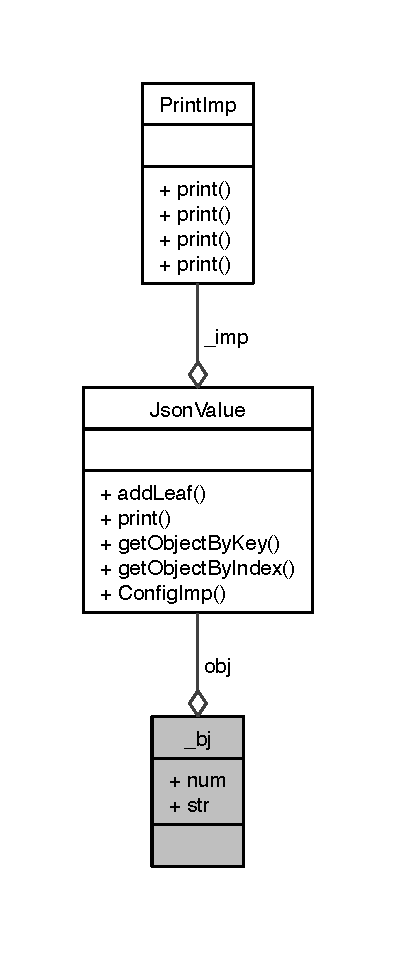
\includegraphics[width=190pt]{struct__bj__coll__graph}
\end{center}
\end{figure}
\subsection*{Public Attributes}
\begin{DoxyCompactItemize}
\item 
\hypertarget{struct__bj_ad8a77a8d790e029cce636b93124f103f}{double {\bfseries num}}\label{struct__bj_ad8a77a8d790e029cce636b93124f103f}

\item 
\hypertarget{struct__bj_a54e511054389a64771b91969852149d9}{string {\bfseries str}}\label{struct__bj_a54e511054389a64771b91969852149d9}

\item 
\hypertarget{struct__bj_a832111969ba497a0a7ab52ae982b671b}{\hyperlink{class_json_value}{Json\-Value} $\ast$ {\bfseries obj}}\label{struct__bj_a832111969ba497a0a7ab52ae982b671b}

\end{DoxyCompactItemize}


The documentation for this struct was generated from the following file\-:\begin{DoxyCompactItemize}
\item 
Json\-Parser.\-tab.\-c\end{DoxyCompactItemize}

\hypertarget{class_concrete_builder}{\section{Concrete\-Builder Class Reference}
\label{class_concrete_builder}\index{Concrete\-Builder@{Concrete\-Builder}}
}


Inheritance diagram for Concrete\-Builder\-:\nopagebreak
\begin{figure}[H]
\begin{center}
\leavevmode
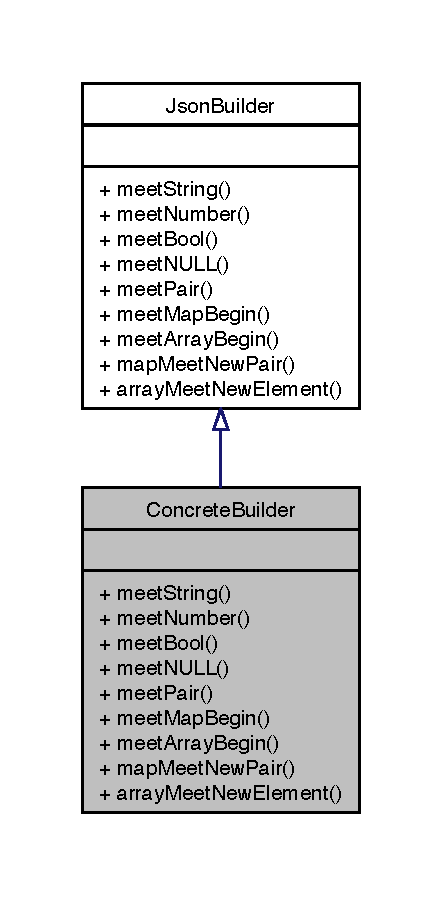
\includegraphics[width=212pt]{class_concrete_builder__inherit__graph}
\end{center}
\end{figure}


Collaboration diagram for Concrete\-Builder\-:\nopagebreak
\begin{figure}[H]
\begin{center}
\leavevmode
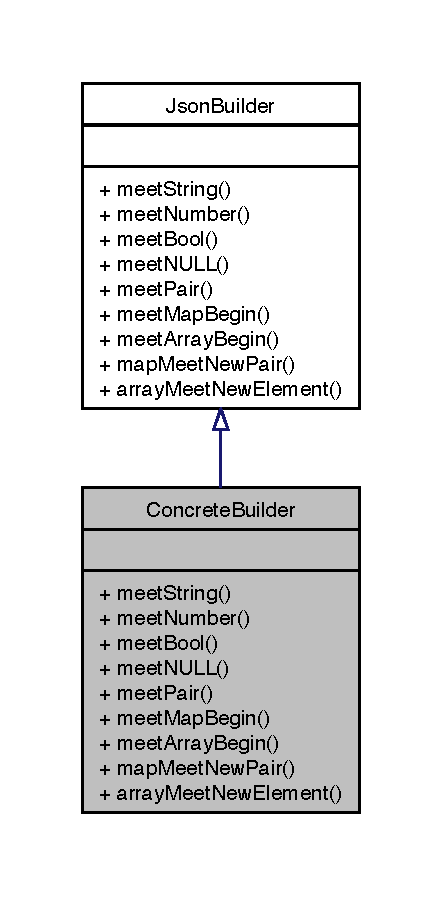
\includegraphics[width=212pt]{class_concrete_builder__coll__graph}
\end{center}
\end{figure}
\subsection*{Public Member Functions}
\begin{DoxyCompactItemize}
\item 
\hypertarget{class_concrete_builder_aa8fc4e3960780086f1447ebf366baf5f}{virtual \hyperlink{class_json_value}{Json\-Value} $\ast$ {\bfseries meet\-String} (std\-::string str)}\label{class_concrete_builder_aa8fc4e3960780086f1447ebf366baf5f}

\item 
\hypertarget{class_concrete_builder_a6391db8468b59761405efccfeb9713a9}{virtual \hyperlink{class_json_value}{Json\-Value} $\ast$ {\bfseries meet\-Number} (double num)}\label{class_concrete_builder_a6391db8468b59761405efccfeb9713a9}

\item 
\hypertarget{class_concrete_builder_a7b10acc7ce30bee8a415f713587bbc23}{virtual \hyperlink{class_json_value}{Json\-Value} $\ast$ {\bfseries meet\-Bool} (bool val)}\label{class_concrete_builder_a7b10acc7ce30bee8a415f713587bbc23}

\item 
\hypertarget{class_concrete_builder_a178b10986703cb7706508284cb7fcb9d}{virtual \hyperlink{class_json_value}{Json\-Value} $\ast$ {\bfseries meet\-N\-U\-L\-L} ()}\label{class_concrete_builder_a178b10986703cb7706508284cb7fcb9d}

\item 
\hypertarget{class_concrete_builder_a87758c86a8e56a3dcd84099fe1a94517}{virtual \hyperlink{class_json_value}{Json\-Value} $\ast$ {\bfseries meet\-Pair} (\hyperlink{class_json_value}{Json\-Value} $\ast$key, \hyperlink{class_json_value}{Json\-Value} $\ast$value)}\label{class_concrete_builder_a87758c86a8e56a3dcd84099fe1a94517}

\item 
\hypertarget{class_concrete_builder_a87ec9354604e496f8cf837970d0c1811}{virtual \hyperlink{class_json_value}{Json\-Value} $\ast$ {\bfseries meet\-Map\-Begin} ()}\label{class_concrete_builder_a87ec9354604e496f8cf837970d0c1811}

\item 
\hypertarget{class_concrete_builder_abd991e1723ecf804ff17a5737d77396f}{virtual \hyperlink{class_json_value}{Json\-Value} $\ast$ {\bfseries meet\-Array\-Begin} ()}\label{class_concrete_builder_abd991e1723ecf804ff17a5737d77396f}

\item 
\hypertarget{class_concrete_builder_aa21350f5f8138b2666294543c1d6b058}{virtual void {\bfseries map\-Meet\-New\-Pair} (\hyperlink{class_json_value}{Json\-Value} $\ast$a\-Map, \hyperlink{class_json_value}{Json\-Value} $\ast$a\-Pair)}\label{class_concrete_builder_aa21350f5f8138b2666294543c1d6b058}

\item 
\hypertarget{class_concrete_builder_a0a0c88e4fd092354206209e96ffb9c13}{virtual void {\bfseries array\-Meet\-New\-Element} (\hyperlink{class_json_value}{Json\-Value} $\ast$array, \hyperlink{class_json_value}{Json\-Value} $\ast$element)}\label{class_concrete_builder_a0a0c88e4fd092354206209e96ffb9c13}

\end{DoxyCompactItemize}


The documentation for this class was generated from the following file\-:\begin{DoxyCompactItemize}
\item 
Concrete\-Builder.\-h\end{DoxyCompactItemize}

\hypertarget{class_data_not_found_exception}{\section{Data\-Not\-Found\-Exception Class Reference}
\label{class_data_not_found_exception}\index{Data\-Not\-Found\-Exception@{Data\-Not\-Found\-Exception}}
}


Inheritance diagram for Data\-Not\-Found\-Exception\-:\nopagebreak
\begin{figure}[H]
\begin{center}
\leavevmode
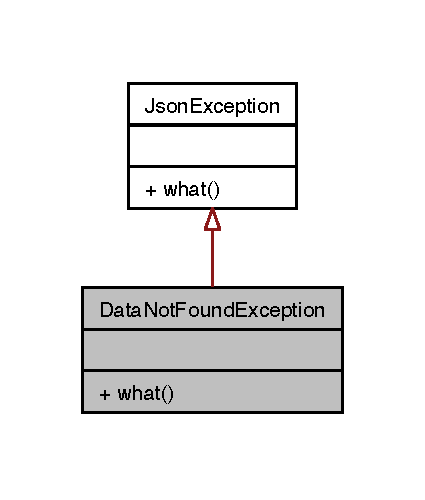
\includegraphics[width=204pt]{class_data_not_found_exception__inherit__graph}
\end{center}
\end{figure}


Collaboration diagram for Data\-Not\-Found\-Exception\-:\nopagebreak
\begin{figure}[H]
\begin{center}
\leavevmode
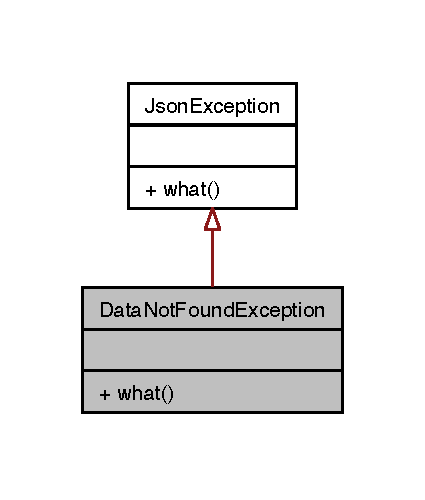
\includegraphics[width=204pt]{class_data_not_found_exception__coll__graph}
\end{center}
\end{figure}
\subsection*{Public Member Functions}
\begin{DoxyCompactItemize}
\item 
\hypertarget{class_data_not_found_exception_adbf1550e8d1f53dbbdac41b8b64a5abe}{virtual const char $\ast$ {\bfseries what} () const   throw ()}\label{class_data_not_found_exception_adbf1550e8d1f53dbbdac41b8b64a5abe}

\end{DoxyCompactItemize}


The documentation for this class was generated from the following files\-:\begin{DoxyCompactItemize}
\item 
Json\-Exception.\-h\item 
Json\-Exception.\-cpp\end{DoxyCompactItemize}

\hypertarget{class_default_print_imp}{\section{Default\-Print\-Imp Class Reference}
\label{class_default_print_imp}\index{Default\-Print\-Imp@{Default\-Print\-Imp}}
}


Inheritance diagram for Default\-Print\-Imp\-:\nopagebreak
\begin{figure}[H]
\begin{center}
\leavevmode
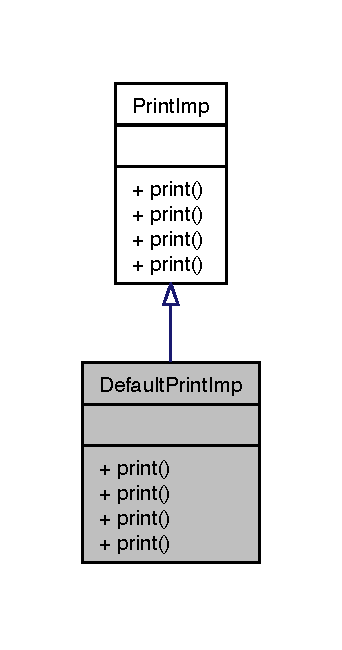
\includegraphics[width=164pt]{class_default_print_imp__inherit__graph}
\end{center}
\end{figure}


Collaboration diagram for Default\-Print\-Imp\-:\nopagebreak
\begin{figure}[H]
\begin{center}
\leavevmode
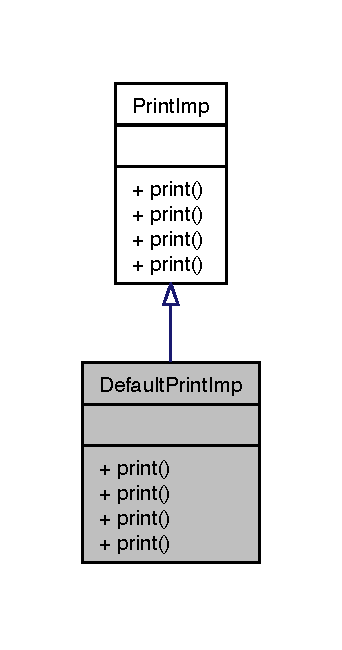
\includegraphics[width=164pt]{class_default_print_imp__coll__graph}
\end{center}
\end{figure}
\subsection*{Public Member Functions}
\begin{DoxyCompactItemize}
\item 
\hypertarget{class_default_print_imp_a3c5e2fe3de894a4a73e80c32c9c635f6}{void {\bfseries print} (ostream \&, \hyperlink{class_json_value}{Json\-Value} $\ast$, int) const }\label{class_default_print_imp_a3c5e2fe3de894a4a73e80c32c9c635f6}

\item 
\hypertarget{class_default_print_imp_ae0e286005fccd96db0fa89284f981581}{void {\bfseries print} (ostream \&, \hyperlink{class_pair}{Pair} $\ast$, int) const }\label{class_default_print_imp_ae0e286005fccd96db0fa89284f981581}

\item 
\hypertarget{class_default_print_imp_ae298ea68db9a0ec325842debb3d47ee6}{void {\bfseries print} (ostream \&, \hyperlink{class_json_object}{Json\-Object} $\ast$, int) const }\label{class_default_print_imp_ae298ea68db9a0ec325842debb3d47ee6}

\item 
\hypertarget{class_default_print_imp_a568dfb4baf46d29ddb0b3f894a08e7e2}{void {\bfseries print} (ostream \&, \hyperlink{class_json_array}{Json\-Array} $\ast$, int) const }\label{class_default_print_imp_a568dfb4baf46d29ddb0b3f894a08e7e2}

\end{DoxyCompactItemize}


The documentation for this class was generated from the following files\-:\begin{DoxyCompactItemize}
\item 
Print\-Imp.\-h\item 
Print\-Imp.\-cpp\end{DoxyCompactItemize}

\hypertarget{class_incorrect_json_exception}{\section{Incorrect\-Json\-Exception Class Reference}
\label{class_incorrect_json_exception}\index{Incorrect\-Json\-Exception@{Incorrect\-Json\-Exception}}
}


Inheritance diagram for Incorrect\-Json\-Exception\-:\nopagebreak
\begin{figure}[H]
\begin{center}
\leavevmode
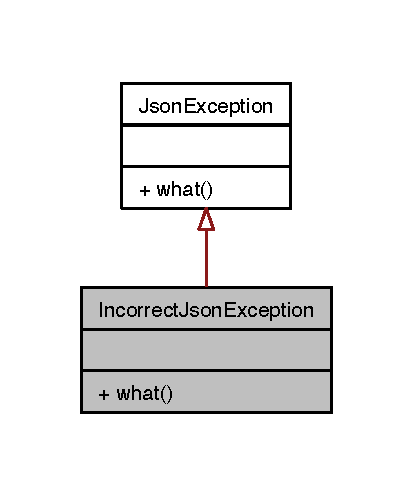
\includegraphics[width=198pt]{class_incorrect_json_exception__inherit__graph}
\end{center}
\end{figure}


Collaboration diagram for Incorrect\-Json\-Exception\-:\nopagebreak
\begin{figure}[H]
\begin{center}
\leavevmode
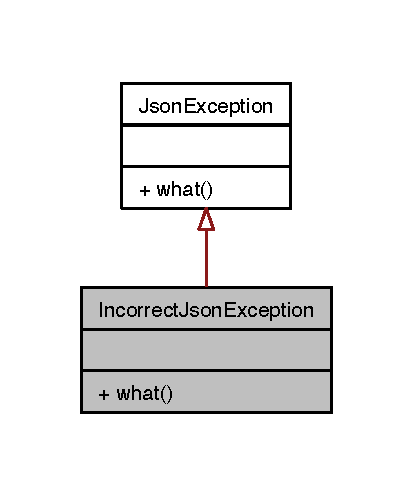
\includegraphics[width=198pt]{class_incorrect_json_exception__coll__graph}
\end{center}
\end{figure}
\subsection*{Public Member Functions}
\begin{DoxyCompactItemize}
\item 
\hypertarget{class_incorrect_json_exception_a53861ce40d8dcf045cca08698d43dea4}{virtual const char $\ast$ {\bfseries what} () const   throw ()}\label{class_incorrect_json_exception_a53861ce40d8dcf045cca08698d43dea4}

\end{DoxyCompactItemize}


The documentation for this class was generated from the following files\-:\begin{DoxyCompactItemize}
\item 
Json\-Exception.\-h\item 
Json\-Exception.\-cpp\end{DoxyCompactItemize}

\hypertarget{class_json_array}{\section{Json\-Array Class Reference}
\label{class_json_array}\index{Json\-Array@{Json\-Array}}
}


Inheritance diagram for Json\-Array\-:
\nopagebreak
\begin{figure}[H]
\begin{center}
\leavevmode
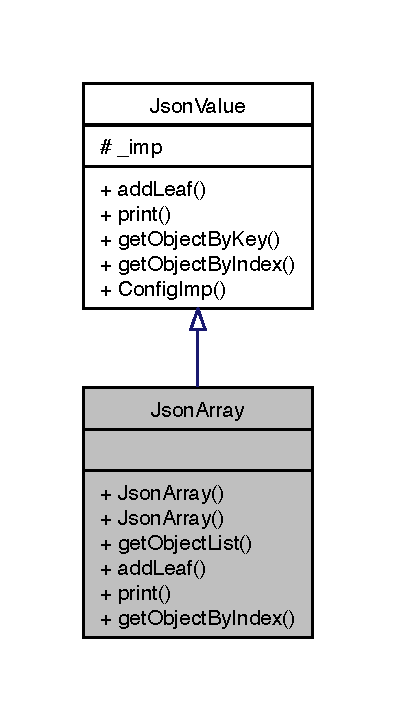
\includegraphics[width=190pt]{class_json_array__inherit__graph}
\end{center}
\end{figure}


Collaboration diagram for Json\-Array\-:
\nopagebreak
\begin{figure}[H]
\begin{center}
\leavevmode
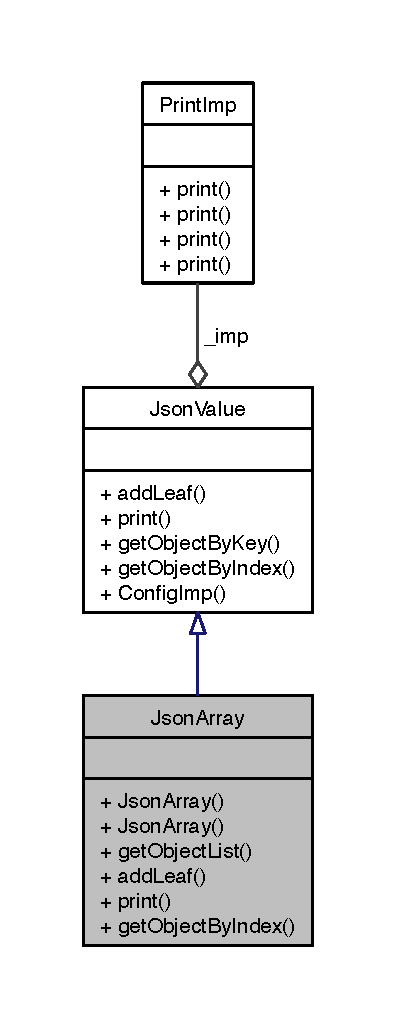
\includegraphics[width=190pt]{class_json_array__coll__graph}
\end{center}
\end{figure}
\subsection*{Public Member Functions}
\begin{DoxyCompactItemize}
\item 
\hyperlink{class_json_array_a304f5ede160dbc87f9ec7d7983bd1cbf}{Json\-Array} ()
\item 
\hypertarget{class_json_array_a4a768c328c454ea855fac1bbb23025fc}{{\bfseries Json\-Array} (const \hyperlink{class_json_array}{Json\-Array} \&rhs)}\label{class_json_array_a4a768c328c454ea855fac1bbb23025fc}

\item 
\hypertarget{class_json_array_a2df7d6f19991476ff0795cb26bd91a53}{vector$<$ \hyperlink{class_json_value}{Json\-Value} $\ast$ $>$ {\bfseries get\-Object\-List} ()}\label{class_json_array_a2df7d6f19991476ff0795cb26bd91a53}

\item 
\hypertarget{class_json_array_ad2ba1e9b80929d31726492539f898b8a}{virtual void {\bfseries add\-Leaf} (\hyperlink{class_json_value}{Json\-Value} $\ast$v)}\label{class_json_array_ad2ba1e9b80929d31726492539f898b8a}

\item 
\hypertarget{class_json_array_a64d9e6d7202141b80a37a9474500fe86}{virtual void {\bfseries print} (ostream \&, int level)}\label{class_json_array_a64d9e6d7202141b80a37a9474500fe86}

\item 
\hypertarget{class_json_array_a3918f99b750f2add69a5c6377df60d74}{virtual \hyperlink{class_json_value}{Json\-Value} $\ast$ {\bfseries get\-Object\-By\-Index} (const int \&index)}\label{class_json_array_a3918f99b750f2add69a5c6377df60d74}

\end{DoxyCompactItemize}


\subsection{Constructor \& Destructor Documentation}
\hypertarget{class_json_array_a304f5ede160dbc87f9ec7d7983bd1cbf}{\index{Json\-Array@{Json\-Array}!Json\-Array@{Json\-Array}}
\index{Json\-Array@{Json\-Array}!JsonArray@{Json\-Array}}
\subsubsection[{Json\-Array}]{\setlength{\rightskip}{0pt plus 5cm}{\bf Json\-Array\-::\-Json\-Array} (
\begin{DoxyParamCaption}
{}
\end{DoxyParamCaption}
)}}\label{class_json_array_a304f5ede160dbc87f9ec7d7983bd1cbf}
\hyperlink{class_json_array}{Json\-Array} 

The documentation for this class was generated from the following files\-:\begin{DoxyCompactItemize}
\item 
Json\-Value.\-h\item 
Json\-Value.\-cpp\end{DoxyCompactItemize}

\hypertarget{class_json_boolean}{\section{Json\-Boolean Class Reference}
\label{class_json_boolean}\index{Json\-Boolean@{Json\-Boolean}}
}


Inheritance diagram for Json\-Boolean\-:
\nopagebreak
\begin{figure}[H]
\begin{center}
\leavevmode
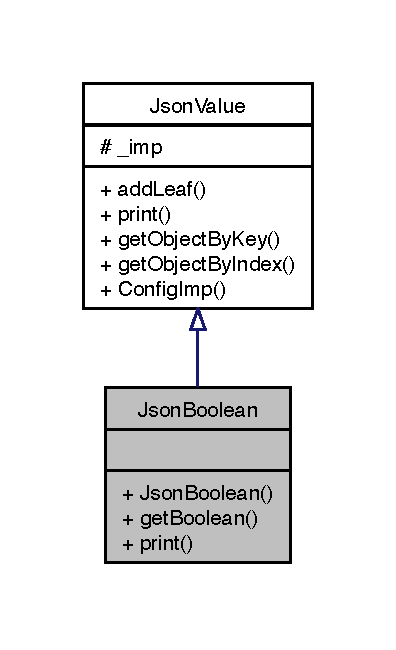
\includegraphics[width=190pt]{class_json_boolean__inherit__graph}
\end{center}
\end{figure}


Collaboration diagram for Json\-Boolean\-:
\nopagebreak
\begin{figure}[H]
\begin{center}
\leavevmode
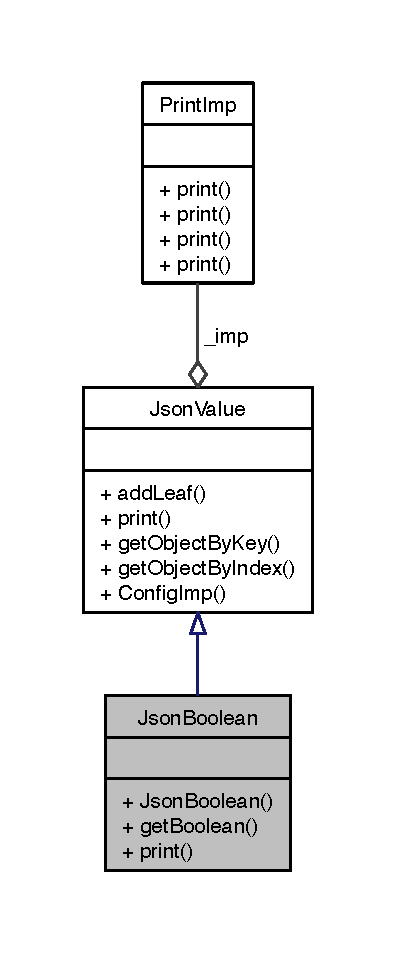
\includegraphics[width=190pt]{class_json_boolean__coll__graph}
\end{center}
\end{figure}
\subsection*{Public Member Functions}
\begin{DoxyCompactItemize}
\item 
\hypertarget{class_json_boolean_acd2c55b733c9f50ff1e6d7f52fa50b31}{{\bfseries Json\-Boolean} (bool b)}\label{class_json_boolean_acd2c55b733c9f50ff1e6d7f52fa50b31}

\item 
\hypertarget{class_json_boolean_ab2015eb0c0029f8a80223a2c3f5106e1}{bool {\bfseries get\-Boolean} ()}\label{class_json_boolean_ab2015eb0c0029f8a80223a2c3f5106e1}

\item 
virtual void \hyperlink{class_json_boolean_a0070f85c41b82ab154897e4f63e8ee37}{print} (ostream \&, int level)
\end{DoxyCompactItemize}


\subsection{Member Function Documentation}
\hypertarget{class_json_boolean_a0070f85c41b82ab154897e4f63e8ee37}{\index{Json\-Boolean@{Json\-Boolean}!print@{print}}
\index{print@{print}!JsonBoolean@{Json\-Boolean}}
\subsubsection[{print}]{\setlength{\rightskip}{0pt plus 5cm}void {\bf Json\-Boolean\-::print} (
\begin{DoxyParamCaption}
\item[{ostream \&}]{os, }
\item[{int}]{level}
\end{DoxyParamCaption}
)\hspace{0.3cm}{\ttfamily  \mbox{[}virtual\mbox{]}}}}\label{class_json_boolean_a0070f85c41b82ab154897e4f63e8ee37}
\hyperlink{class_json_boolean}{Json\-Boolean} 

Reimplemented from \hyperlink{class_json_value}{Json\-Value}.



The documentation for this class was generated from the following files\-:\begin{DoxyCompactItemize}
\item 
Json\-Value.\-h\item 
Json\-Value.\-cpp\end{DoxyCompactItemize}

\hypertarget{class_json_builder}{\section{Json\-Builder Class Reference}
\label{class_json_builder}\index{Json\-Builder@{Json\-Builder}}
}


Inheritance diagram for Json\-Builder\-:\nopagebreak
\begin{figure}[H]
\begin{center}
\leavevmode
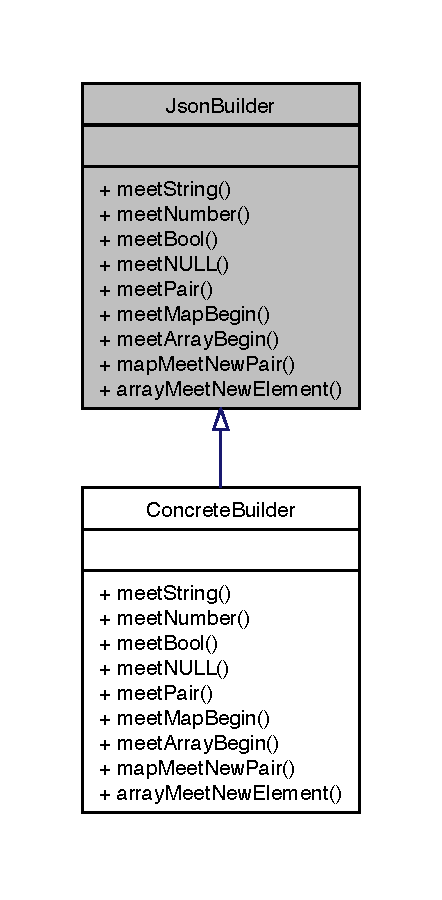
\includegraphics[width=212pt]{class_json_builder__inherit__graph}
\end{center}
\end{figure}
\subsection*{Public Member Functions}
\begin{DoxyCompactItemize}
\item 
\hypertarget{class_json_builder_a360f25eb3df72b07d7a0f0cad619fc01}{virtual \hyperlink{class_json_value}{Json\-Value} $\ast$ {\bfseries meet\-String} (std\-::string str)=0}\label{class_json_builder_a360f25eb3df72b07d7a0f0cad619fc01}

\item 
\hypertarget{class_json_builder_a5b1161dce599fd377786412427a7bbfd}{virtual \hyperlink{class_json_value}{Json\-Value} $\ast$ {\bfseries meet\-Number} (double num)=0}\label{class_json_builder_a5b1161dce599fd377786412427a7bbfd}

\item 
\hypertarget{class_json_builder_ac8b310cf6ae1f98a3984d647204ae758}{virtual \hyperlink{class_json_value}{Json\-Value} $\ast$ {\bfseries meet\-Bool} (bool val)=0}\label{class_json_builder_ac8b310cf6ae1f98a3984d647204ae758}

\item 
\hypertarget{class_json_builder_a189a522b3de4ac4d93f255edf5362846}{virtual \hyperlink{class_json_value}{Json\-Value} $\ast$ {\bfseries meet\-N\-U\-L\-L} ()=0}\label{class_json_builder_a189a522b3de4ac4d93f255edf5362846}

\item 
\hypertarget{class_json_builder_a570f09a130ba19238ef8fb76c2c50902}{virtual \hyperlink{class_json_value}{Json\-Value} $\ast$ {\bfseries meet\-Pair} (\hyperlink{class_json_value}{Json\-Value} $\ast$key, \hyperlink{class_json_value}{Json\-Value} $\ast$value)=0}\label{class_json_builder_a570f09a130ba19238ef8fb76c2c50902}

\item 
\hypertarget{class_json_builder_ad5fe8e884e409cef76b86d938f9afca5}{virtual \hyperlink{class_json_value}{Json\-Value} $\ast$ {\bfseries meet\-Map\-Begin} ()=0}\label{class_json_builder_ad5fe8e884e409cef76b86d938f9afca5}

\item 
\hypertarget{class_json_builder_a0547b28bac563a3a587071b108e84159}{virtual \hyperlink{class_json_value}{Json\-Value} $\ast$ {\bfseries meet\-Array\-Begin} ()=0}\label{class_json_builder_a0547b28bac563a3a587071b108e84159}

\item 
\hypertarget{class_json_builder_ad09c1859ff1383b1081317f2626079ff}{virtual void {\bfseries map\-Meet\-New\-Pair} (\hyperlink{class_json_value}{Json\-Value} $\ast$map, \hyperlink{class_json_value}{Json\-Value} $\ast$pair)}\label{class_json_builder_ad09c1859ff1383b1081317f2626079ff}

\item 
\hypertarget{class_json_builder_a5bab3a246addf149c3bfd311e5179c11}{virtual void {\bfseries array\-Meet\-New\-Element} (\hyperlink{class_json_value}{Json\-Value} $\ast$array, \hyperlink{class_json_value}{Json\-Value} $\ast$element)}\label{class_json_builder_a5bab3a246addf149c3bfd311e5179c11}

\end{DoxyCompactItemize}


The documentation for this class was generated from the following file\-:\begin{DoxyCompactItemize}
\item 
Json\-Builder.\-h\end{DoxyCompactItemize}

\hypertarget{class_json_double}{\section{Json\-Double Class Reference}
\label{class_json_double}\index{Json\-Double@{Json\-Double}}
}


Inheritance diagram for Json\-Double\-:
\nopagebreak
\begin{figure}[H]
\begin{center}
\leavevmode
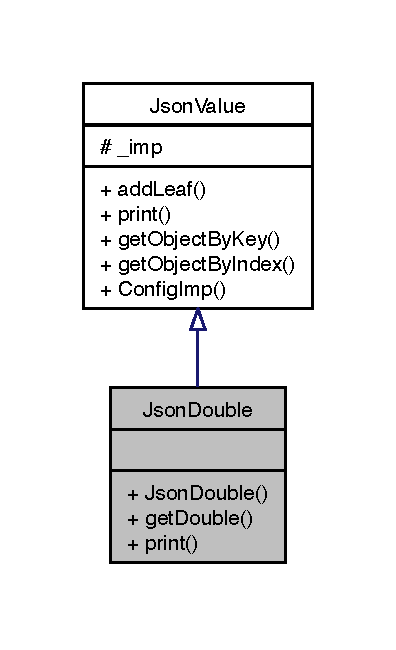
\includegraphics[width=190pt]{class_json_double__inherit__graph}
\end{center}
\end{figure}


Collaboration diagram for Json\-Double\-:
\nopagebreak
\begin{figure}[H]
\begin{center}
\leavevmode
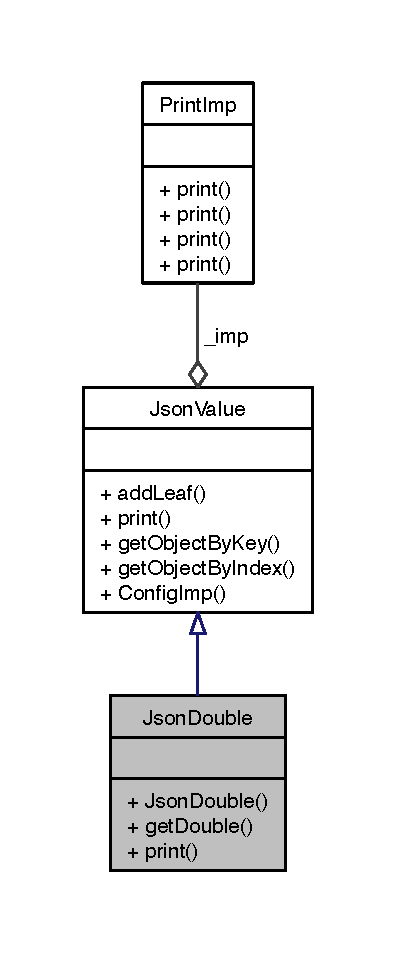
\includegraphics[width=190pt]{class_json_double__coll__graph}
\end{center}
\end{figure}
\subsection*{Public Member Functions}
\begin{DoxyCompactItemize}
\item 
\hypertarget{class_json_double_a3171538496cf69c6e613d57fb43bb692}{{\bfseries Json\-Double} (double d)}\label{class_json_double_a3171538496cf69c6e613d57fb43bb692}

\item 
\hypertarget{class_json_double_a97a624d311e723499244fab443fe7699}{double {\bfseries get\-Double} ()}\label{class_json_double_a97a624d311e723499244fab443fe7699}

\item 
virtual void \hyperlink{class_json_double_ada04ed5065552f926e67fbea530dced5}{print} (ostream \&, int level)
\end{DoxyCompactItemize}


\subsection{Member Function Documentation}
\hypertarget{class_json_double_ada04ed5065552f926e67fbea530dced5}{\index{Json\-Double@{Json\-Double}!print@{print}}
\index{print@{print}!JsonDouble@{Json\-Double}}
\subsubsection[{print}]{\setlength{\rightskip}{0pt plus 5cm}void {\bf Json\-Double\-::print} (
\begin{DoxyParamCaption}
\item[{ostream \&}]{os, }
\item[{int}]{level}
\end{DoxyParamCaption}
)\hspace{0.3cm}{\ttfamily  \mbox{[}virtual\mbox{]}}}}\label{class_json_double_ada04ed5065552f926e67fbea530dced5}
\hyperlink{class_json_double}{Json\-Double} 

Reimplemented from \hyperlink{class_json_value}{Json\-Value}.



The documentation for this class was generated from the following files\-:\begin{DoxyCompactItemize}
\item 
Json\-Value.\-h\item 
Json\-Value.\-cpp\end{DoxyCompactItemize}

\hypertarget{class_json_exception}{\section{Json\-Exception Class Reference}
\label{class_json_exception}\index{Json\-Exception@{Json\-Exception}}
}


Inheritance diagram for Json\-Exception\-:\nopagebreak
\begin{figure}[H]
\begin{center}
\leavevmode
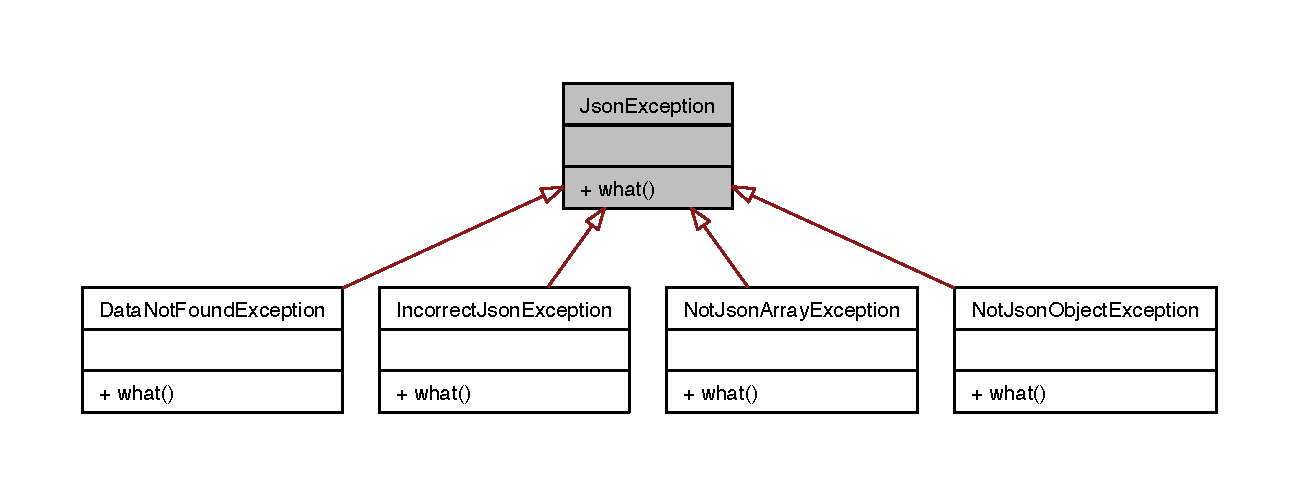
\includegraphics[width=350pt]{class_json_exception__inherit__graph}
\end{center}
\end{figure}
\subsection*{Public Member Functions}
\begin{DoxyCompactItemize}
\item 
\hypertarget{class_json_exception_a964d4111c787ab522aff9725bf129e52}{virtual const char $\ast$ {\bfseries what} () const   throw ()}\label{class_json_exception_a964d4111c787ab522aff9725bf129e52}

\end{DoxyCompactItemize}


The documentation for this class was generated from the following files\-:\begin{DoxyCompactItemize}
\item 
Json\-Exception.\-h\item 
Json\-Exception.\-cpp\end{DoxyCompactItemize}

\hypertarget{class_json_null}{\section{Json\-Null Class Reference}
\label{class_json_null}\index{Json\-Null@{Json\-Null}}
}


Inheritance diagram for Json\-Null\-:
\nopagebreak
\begin{figure}[H]
\begin{center}
\leavevmode
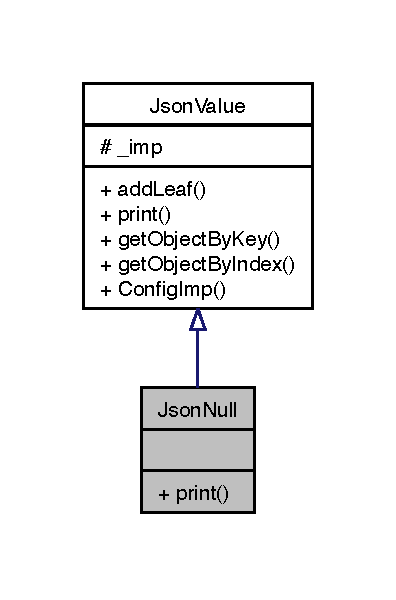
\includegraphics[width=190pt]{class_json_null__inherit__graph}
\end{center}
\end{figure}


Collaboration diagram for Json\-Null\-:
\nopagebreak
\begin{figure}[H]
\begin{center}
\leavevmode
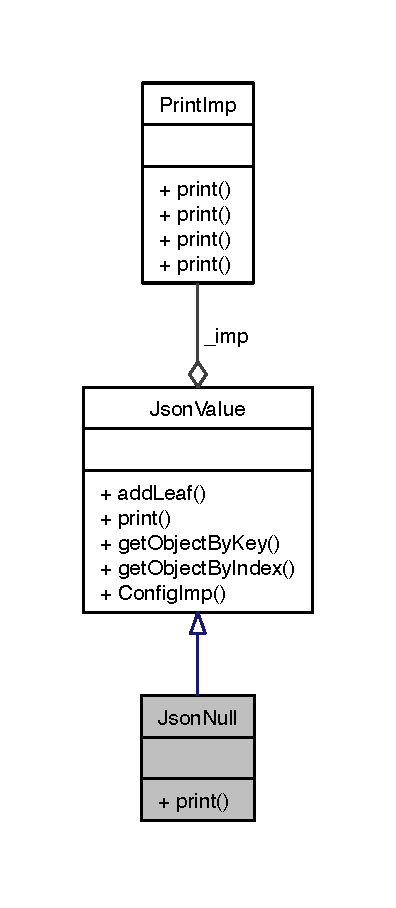
\includegraphics[width=190pt]{class_json_null__coll__graph}
\end{center}
\end{figure}
\subsection*{Public Member Functions}
\begin{DoxyCompactItemize}
\item 
virtual void \hyperlink{class_json_null_a02e120cf518f258b134ea21051d2a2d6}{print} (ostream \&, int level)
\end{DoxyCompactItemize}


\subsection{Member Function Documentation}
\hypertarget{class_json_null_a02e120cf518f258b134ea21051d2a2d6}{\index{Json\-Null@{Json\-Null}!print@{print}}
\index{print@{print}!JsonNull@{Json\-Null}}
\subsubsection[{print}]{\setlength{\rightskip}{0pt plus 5cm}void {\bf Json\-Null\-::print} (
\begin{DoxyParamCaption}
\item[{ostream \&}]{os, }
\item[{int}]{level}
\end{DoxyParamCaption}
)\hspace{0.3cm}{\ttfamily  \mbox{[}virtual\mbox{]}}}}\label{class_json_null_a02e120cf518f258b134ea21051d2a2d6}
\hyperlink{class_json_null}{Json\-Null} 

Reimplemented from \hyperlink{class_json_value}{Json\-Value}.



The documentation for this class was generated from the following files\-:\begin{DoxyCompactItemize}
\item 
Json\-Value.\-h\item 
Json\-Value.\-cpp\end{DoxyCompactItemize}

\hypertarget{class_json_object}{\section{Json\-Object Class Reference}
\label{class_json_object}\index{Json\-Object@{Json\-Object}}
}


Inheritance diagram for Json\-Object\-:
\nopagebreak
\begin{figure}[H]
\begin{center}
\leavevmode
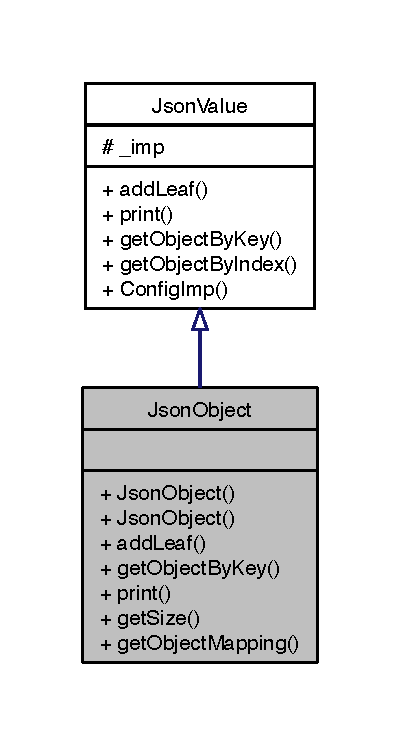
\includegraphics[width=192pt]{class_json_object__inherit__graph}
\end{center}
\end{figure}


Collaboration diagram for Json\-Object\-:
\nopagebreak
\begin{figure}[H]
\begin{center}
\leavevmode
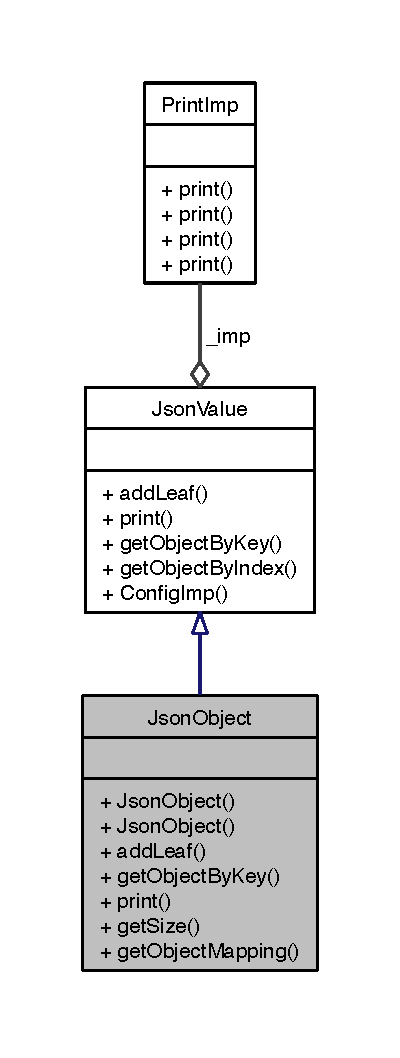
\includegraphics[width=192pt]{class_json_object__coll__graph}
\end{center}
\end{figure}
\subsection*{Public Types}
\begin{DoxyCompactItemize}
\item 
\hypertarget{class_json_object_a83a1255aafe7ac715e6a252e5f3f95b9}{typedef map$<$ string, \hyperlink{class_json_value}{Json\-Value} $\ast$ $>$ {\bfseries J\-S\-O\-N\-\_\-\-O\-B\-J\-E\-C\-T}}\label{class_json_object_a83a1255aafe7ac715e6a252e5f3f95b9}

\end{DoxyCompactItemize}
\subsection*{Public Member Functions}
\begin{DoxyCompactItemize}
\item 
\hyperlink{class_json_object_aa41d053fc27e4fcf4f1c6f55ef28f4a9}{Json\-Object} ()
\item 
\hypertarget{class_json_object_ae73160f77eda4c46b170dded5c18deb1}{{\bfseries Json\-Object} (const \hyperlink{class_json_object}{Json\-Object} \&rhs)}\label{class_json_object_ae73160f77eda4c46b170dded5c18deb1}

\item 
\hypertarget{class_json_object_abeb76c4a8e916b910d26c0e28f104539}{virtual void {\bfseries add\-Leaf} (\hyperlink{class_json_value}{Json\-Value} $\ast$v)}\label{class_json_object_abeb76c4a8e916b910d26c0e28f104539}

\item 
\hypertarget{class_json_object_a9f9a1c3ed146aad941f78ff39fc8539c}{virtual \hyperlink{class_json_value}{Json\-Value} $\ast$ {\bfseries get\-Object\-By\-Key} (const string \&key)}\label{class_json_object_a9f9a1c3ed146aad941f78ff39fc8539c}

\item 
\hypertarget{class_json_object_a46c41a321e894dad5116697dc337b560}{virtual void {\bfseries print} (ostream \&, int level)}\label{class_json_object_a46c41a321e894dad5116697dc337b560}

\item 
\hypertarget{class_json_object_ade653098d46f75ff35a27a83bf5b8c51}{int {\bfseries get\-Size} ()}\label{class_json_object_ade653098d46f75ff35a27a83bf5b8c51}

\item 
\hypertarget{class_json_object_a98aea612e8f5251c96213b9b74ea62f9}{J\-S\-O\-N\-\_\-\-O\-B\-J\-E\-C\-T {\bfseries get\-Object\-Mapping} ()}\label{class_json_object_a98aea612e8f5251c96213b9b74ea62f9}

\end{DoxyCompactItemize}


\subsection{Constructor \& Destructor Documentation}
\hypertarget{class_json_object_aa41d053fc27e4fcf4f1c6f55ef28f4a9}{\index{Json\-Object@{Json\-Object}!Json\-Object@{Json\-Object}}
\index{Json\-Object@{Json\-Object}!JsonObject@{Json\-Object}}
\subsubsection[{Json\-Object}]{\setlength{\rightskip}{0pt plus 5cm}{\bf Json\-Object\-::\-Json\-Object} (
\begin{DoxyParamCaption}
{}
\end{DoxyParamCaption}
)}}\label{class_json_object_aa41d053fc27e4fcf4f1c6f55ef28f4a9}
\hyperlink{class_json_object}{Json\-Object} 

The documentation for this class was generated from the following files\-:\begin{DoxyCompactItemize}
\item 
Json\-Value.\-h\item 
Json\-Value.\-cpp\end{DoxyCompactItemize}

\hypertarget{class_json_string}{\section{Json\-String Class Reference}
\label{class_json_string}\index{Json\-String@{Json\-String}}
}


Inheritance diagram for Json\-String\-:
\nopagebreak
\begin{figure}[H]
\begin{center}
\leavevmode
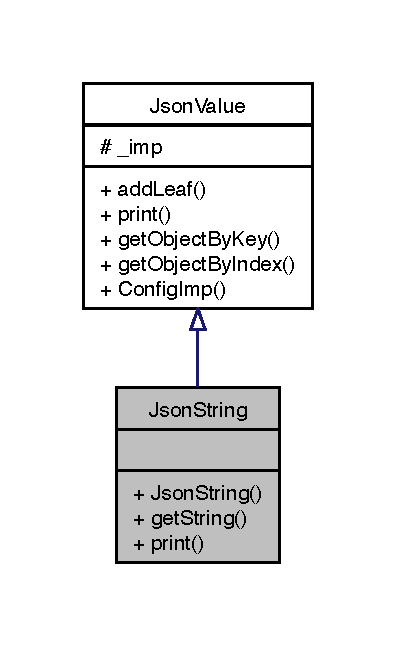
\includegraphics[width=190pt]{class_json_string__inherit__graph}
\end{center}
\end{figure}


Collaboration diagram for Json\-String\-:
\nopagebreak
\begin{figure}[H]
\begin{center}
\leavevmode
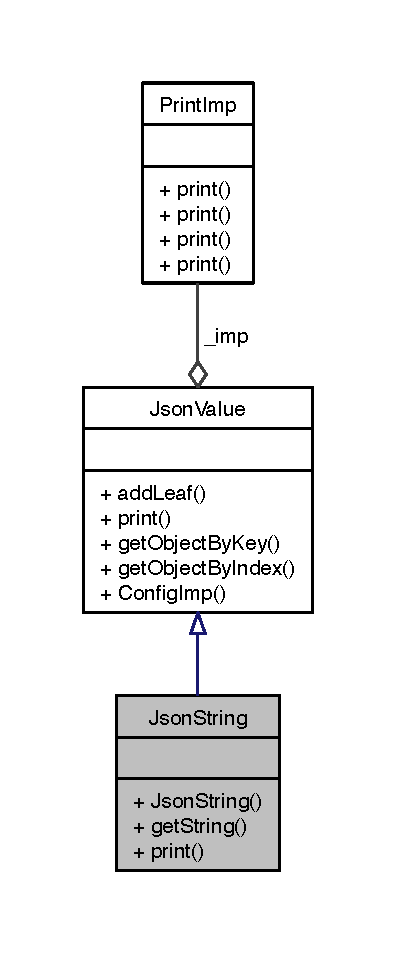
\includegraphics[width=190pt]{class_json_string__coll__graph}
\end{center}
\end{figure}
\subsection*{Public Member Functions}
\begin{DoxyCompactItemize}
\item 
\hypertarget{class_json_string_a1d8dbaf53c0b7b00a0e70ccbe9060131}{{\bfseries Json\-String} (string s)}\label{class_json_string_a1d8dbaf53c0b7b00a0e70ccbe9060131}

\item 
\hypertarget{class_json_string_a029c7f1952a1802288928bee2e454ca8}{string {\bfseries get\-String} ()}\label{class_json_string_a029c7f1952a1802288928bee2e454ca8}

\item 
virtual void \hyperlink{class_json_string_a9d0bb2aa5c210f1eaf6612a4176ee1e0}{print} (ostream \&, int level)
\end{DoxyCompactItemize}


\subsection{Member Function Documentation}
\hypertarget{class_json_string_a9d0bb2aa5c210f1eaf6612a4176ee1e0}{\index{Json\-String@{Json\-String}!print@{print}}
\index{print@{print}!JsonString@{Json\-String}}
\subsubsection[{print}]{\setlength{\rightskip}{0pt plus 5cm}void {\bf Json\-String\-::print} (
\begin{DoxyParamCaption}
\item[{ostream \&}]{os, }
\item[{int}]{level}
\end{DoxyParamCaption}
)\hspace{0.3cm}{\ttfamily  \mbox{[}virtual\mbox{]}}}}\label{class_json_string_a9d0bb2aa5c210f1eaf6612a4176ee1e0}
\hyperlink{class_json_string}{Json\-String} 

Reimplemented from \hyperlink{class_json_value}{Json\-Value}.



The documentation for this class was generated from the following files\-:\begin{DoxyCompactItemize}
\item 
Json\-Value.\-h\item 
Json\-Value.\-cpp\end{DoxyCompactItemize}

\hypertarget{class_json_value}{\section{Json\-Value Class Reference}
\label{class_json_value}\index{Json\-Value@{Json\-Value}}
}


Inheritance diagram for Json\-Value\-:
\nopagebreak
\begin{figure}[H]
\begin{center}
\leavevmode
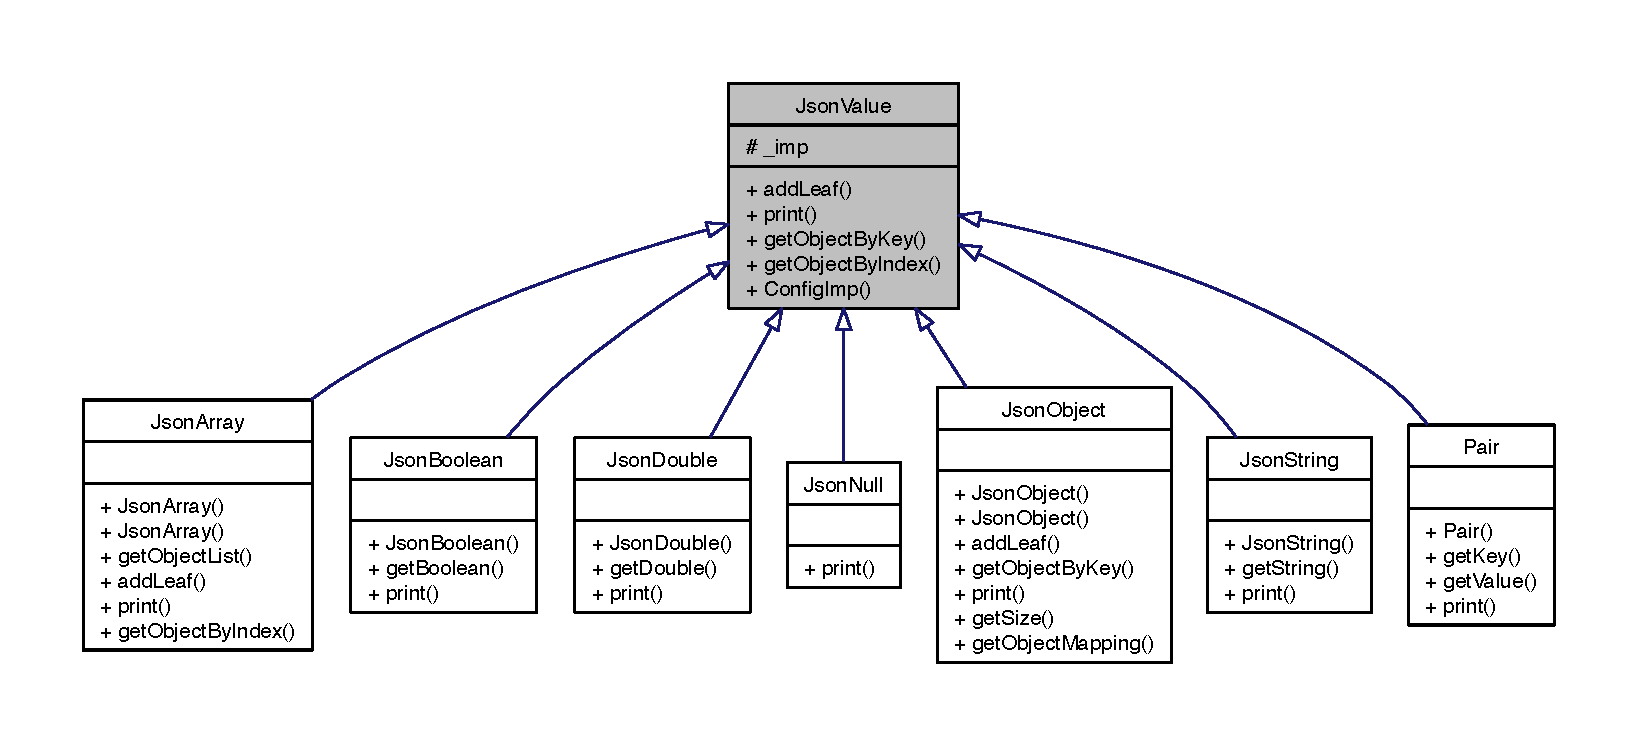
\includegraphics[width=350pt]{class_json_value__inherit__graph}
\end{center}
\end{figure}


Collaboration diagram for Json\-Value\-:
\nopagebreak
\begin{figure}[H]
\begin{center}
\leavevmode
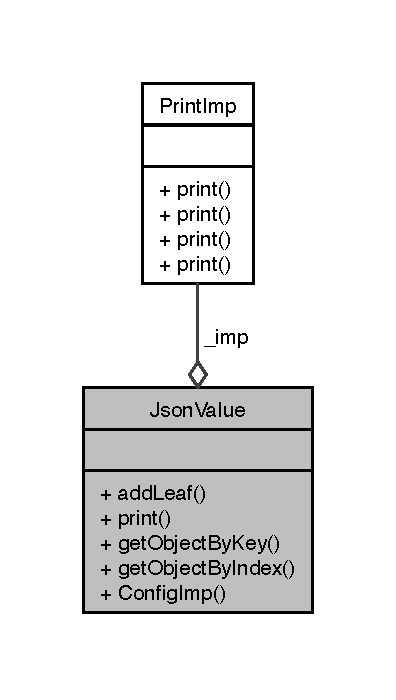
\includegraphics[width=190pt]{class_json_value__coll__graph}
\end{center}
\end{figure}
\subsection*{Public Member Functions}
\begin{DoxyCompactItemize}
\item 
\hypertarget{class_json_value_a7a2553501c656b8dd5bd2803a0a70623}{virtual void {\bfseries add\-Leaf} (\hyperlink{class_json_value}{Json\-Value} $\ast$v)}\label{class_json_value_a7a2553501c656b8dd5bd2803a0a70623}

\item 
\hypertarget{class_json_value_a3f3d41930cd53a7f01cf8bfc7d5374f2}{virtual void {\bfseries print} (ostream \&, int level)}\label{class_json_value_a3f3d41930cd53a7f01cf8bfc7d5374f2}

\item 
\hypertarget{class_json_value_a2d7aa05f7ff5a0749bcd1806ab772b52}{virtual \hyperlink{class_json_value}{Json\-Value} $\ast$ {\bfseries get\-Object\-By\-Key} (const string \&key)}\label{class_json_value_a2d7aa05f7ff5a0749bcd1806ab772b52}

\item 
\hypertarget{class_json_value_a3ce0f88e789d84741805f45426b23263}{virtual \hyperlink{class_json_value}{Json\-Value} $\ast$ {\bfseries get\-Object\-By\-Index} (const int \&index)}\label{class_json_value_a3ce0f88e789d84741805f45426b23263}

\end{DoxyCompactItemize}
\subsection*{Static Public Member Functions}
\begin{DoxyCompactItemize}
\item 
\hypertarget{class_json_value_ad33b6639ae540eb58e4dddd6482e2c2d}{static void {\bfseries Config\-Imp} (\hyperlink{class_print_imp}{Print\-Imp} $\ast$imp)}\label{class_json_value_ad33b6639ae540eb58e4dddd6482e2c2d}

\end{DoxyCompactItemize}
\subsection*{Static Protected Attributes}
\begin{DoxyCompactItemize}
\item 
\hypertarget{class_json_value_adfbf245f1cc2660e840cd7a4d43296c8}{static \hyperlink{class_print_imp}{Print\-Imp} $\ast$ {\bfseries \-\_\-imp}}\label{class_json_value_adfbf245f1cc2660e840cd7a4d43296c8}

\end{DoxyCompactItemize}
\subsection*{Friends}
\begin{DoxyCompactItemize}
\item 
\hypertarget{class_json_value_ad653d7351669da553bc36ba709d5faa5}{ostream \& {\bfseries operator$<$$<$} (ostream \&os, \hyperlink{class_json_value}{Json\-Value} $\ast$v)}\label{class_json_value_ad653d7351669da553bc36ba709d5faa5}

\end{DoxyCompactItemize}


The documentation for this class was generated from the following files\-:\begin{DoxyCompactItemize}
\item 
Json\-Value.\-h\item 
Json\-Value.\-cpp\end{DoxyCompactItemize}

\hypertarget{class_not_json_array_exception}{\section{Not\-Json\-Array\-Exception Class Reference}
\label{class_not_json_array_exception}\index{Not\-Json\-Array\-Exception@{Not\-Json\-Array\-Exception}}
}


Inheritance diagram for Not\-Json\-Array\-Exception\-:\nopagebreak
\begin{figure}[H]
\begin{center}
\leavevmode
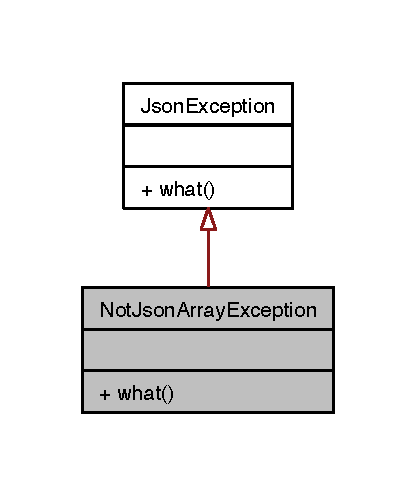
\includegraphics[width=200pt]{class_not_json_array_exception__inherit__graph}
\end{center}
\end{figure}


Collaboration diagram for Not\-Json\-Array\-Exception\-:\nopagebreak
\begin{figure}[H]
\begin{center}
\leavevmode
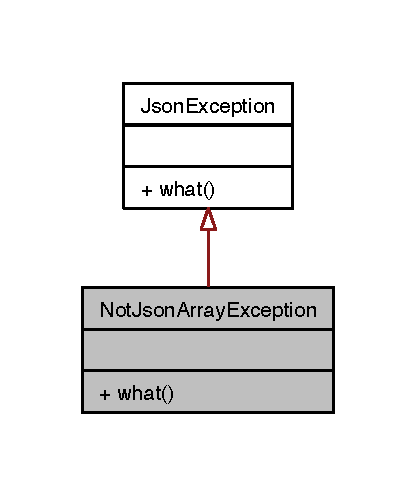
\includegraphics[width=200pt]{class_not_json_array_exception__coll__graph}
\end{center}
\end{figure}
\subsection*{Public Member Functions}
\begin{DoxyCompactItemize}
\item 
\hypertarget{class_not_json_array_exception_af73718295234b7fa370ee6a7ceb0b95e}{virtual const char $\ast$ {\bfseries what} () const   throw ()}\label{class_not_json_array_exception_af73718295234b7fa370ee6a7ceb0b95e}

\end{DoxyCompactItemize}


The documentation for this class was generated from the following files\-:\begin{DoxyCompactItemize}
\item 
Json\-Exception.\-h\item 
Json\-Exception.\-cpp\end{DoxyCompactItemize}

\hypertarget{class_not_json_object_exception}{\section{Not\-Json\-Object\-Exception Class Reference}
\label{class_not_json_object_exception}\index{Not\-Json\-Object\-Exception@{Not\-Json\-Object\-Exception}}
}


Inheritance diagram for Not\-Json\-Object\-Exception\-:\nopagebreak
\begin{figure}[H]
\begin{center}
\leavevmode
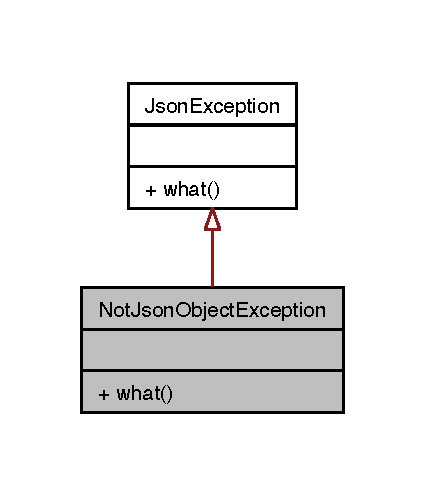
\includegraphics[width=204pt]{class_not_json_object_exception__inherit__graph}
\end{center}
\end{figure}


Collaboration diagram for Not\-Json\-Object\-Exception\-:\nopagebreak
\begin{figure}[H]
\begin{center}
\leavevmode
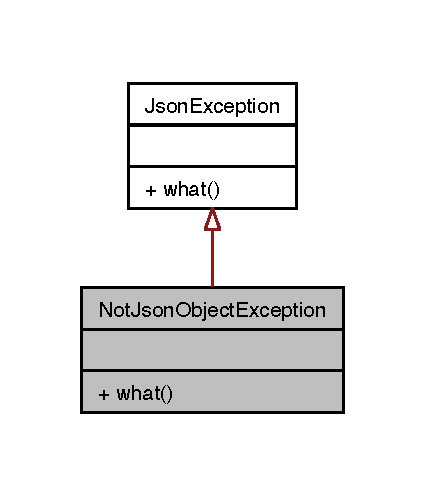
\includegraphics[width=204pt]{class_not_json_object_exception__coll__graph}
\end{center}
\end{figure}
\subsection*{Public Member Functions}
\begin{DoxyCompactItemize}
\item 
\hypertarget{class_not_json_object_exception_a232cc8f09b24e095d416df0242381881}{virtual const char $\ast$ {\bfseries what} () const   throw ()}\label{class_not_json_object_exception_a232cc8f09b24e095d416df0242381881}

\end{DoxyCompactItemize}


The documentation for this class was generated from the following files\-:\begin{DoxyCompactItemize}
\item 
Json\-Exception.\-h\item 
Json\-Exception.\-cpp\end{DoxyCompactItemize}

\hypertarget{class_pair}{\section{Pair Class Reference}
\label{class_pair}\index{Pair@{Pair}}
}


Inheritance diagram for Pair\-:
\nopagebreak
\begin{figure}[H]
\begin{center}
\leavevmode
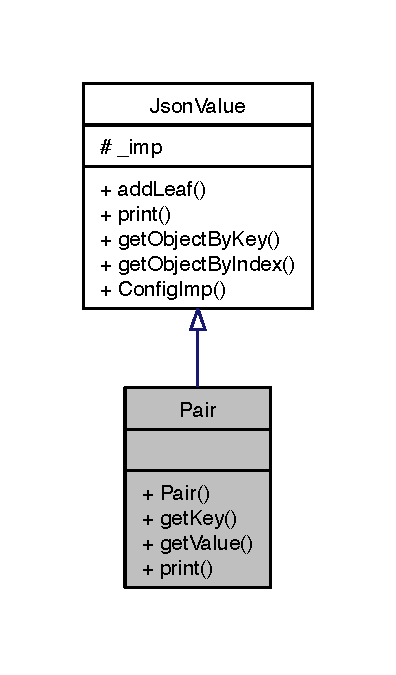
\includegraphics[width=190pt]{class_pair__inherit__graph}
\end{center}
\end{figure}


Collaboration diagram for Pair\-:
\nopagebreak
\begin{figure}[H]
\begin{center}
\leavevmode
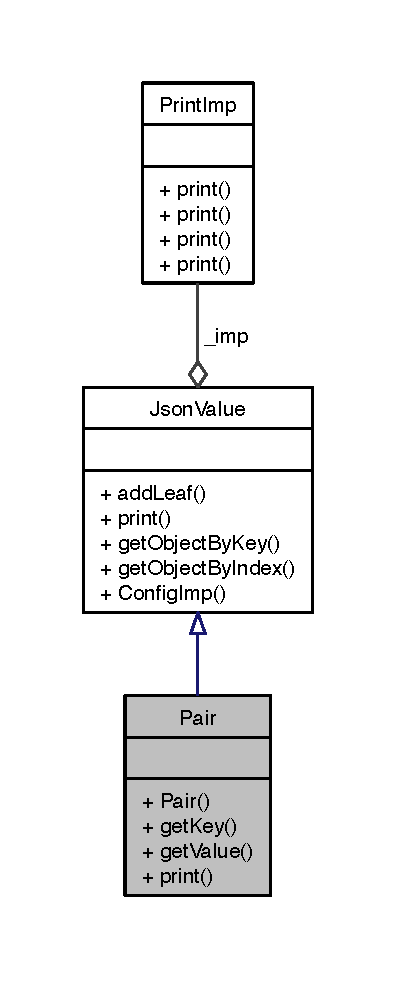
\includegraphics[width=190pt]{class_pair__coll__graph}
\end{center}
\end{figure}
\subsection*{Public Member Functions}
\begin{DoxyCompactItemize}
\item 
\hyperlink{class_pair_ac676514d7dda7fd6105e0f12621ab987}{Pair} (string \&key, \hyperlink{class_json_value}{Json\-Value} $\ast$value)
\item 
\hypertarget{class_pair_af8c963d643601af49efd0407e8482283}{string \& {\bfseries get\-Key} ()}\label{class_pair_af8c963d643601af49efd0407e8482283}

\item 
\hypertarget{class_pair_a3b2b13180c67bd90038a094f05a1b109}{\hyperlink{class_json_value}{Json\-Value} $\ast$ {\bfseries get\-Value} ()}\label{class_pair_a3b2b13180c67bd90038a094f05a1b109}

\item 
\hypertarget{class_pair_a5b2db35455fdfa2a41a80d0381d6b55c}{virtual void {\bfseries print} (ostream \&, int level)}\label{class_pair_a5b2db35455fdfa2a41a80d0381d6b55c}

\end{DoxyCompactItemize}


\subsection{Constructor \& Destructor Documentation}
\hypertarget{class_pair_ac676514d7dda7fd6105e0f12621ab987}{\index{Pair@{Pair}!Pair@{Pair}}
\index{Pair@{Pair}!Pair@{Pair}}
\subsubsection[{Pair}]{\setlength{\rightskip}{0pt plus 5cm}{\bf Pair\-::\-Pair} (
\begin{DoxyParamCaption}
\item[{string \&}]{key, }
\item[{{\bf Json\-Value} $\ast$}]{value}
\end{DoxyParamCaption}
)}}\label{class_pair_ac676514d7dda7fd6105e0f12621ab987}
\hyperlink{class_pair}{Pair} 

The documentation for this class was generated from the following files\-:\begin{DoxyCompactItemize}
\item 
Json\-Value.\-h\item 
Json\-Value.\-cpp\end{DoxyCompactItemize}

\hypertarget{class_pretty_print_imp}{\section{Pretty\-Print\-Imp Class Reference}
\label{class_pretty_print_imp}\index{Pretty\-Print\-Imp@{Pretty\-Print\-Imp}}
}


Inheritance diagram for Pretty\-Print\-Imp\-:\nopagebreak
\begin{figure}[H]
\begin{center}
\leavevmode
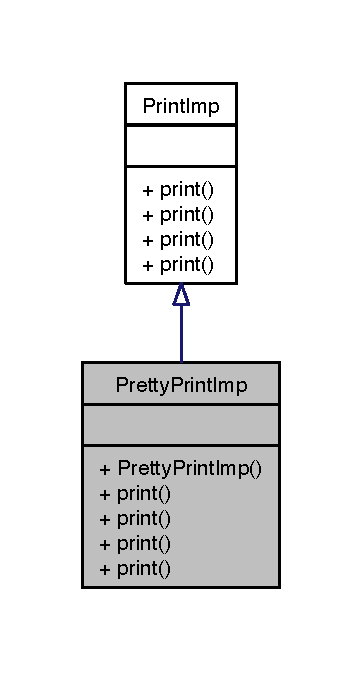
\includegraphics[width=174pt]{class_pretty_print_imp__inherit__graph}
\end{center}
\end{figure}


Collaboration diagram for Pretty\-Print\-Imp\-:\nopagebreak
\begin{figure}[H]
\begin{center}
\leavevmode
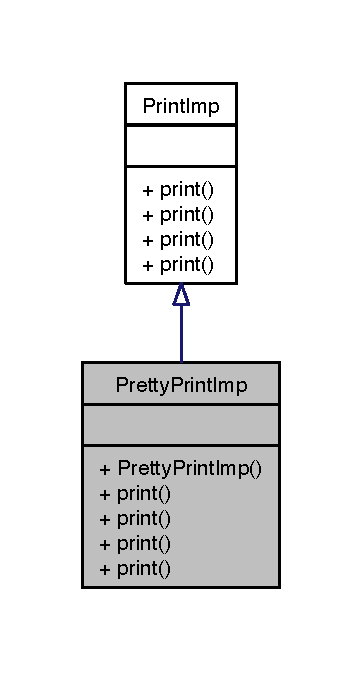
\includegraphics[width=174pt]{class_pretty_print_imp__coll__graph}
\end{center}
\end{figure}
\subsection*{Public Member Functions}
\begin{DoxyCompactItemize}
\item 
\hypertarget{class_pretty_print_imp_a879f3bbe60fe6e3b402bb36ce08275f4}{{\bfseries Pretty\-Print\-Imp} (int sep)}\label{class_pretty_print_imp_a879f3bbe60fe6e3b402bb36ce08275f4}

\item 
\hypertarget{class_pretty_print_imp_a61f4a7aaa44441f990e8dac892de087e}{void {\bfseries print} (ostream \&, \hyperlink{class_json_value}{Json\-Value} $\ast$, int) const }\label{class_pretty_print_imp_a61f4a7aaa44441f990e8dac892de087e}

\item 
\hypertarget{class_pretty_print_imp_ad7217f95b4f8d520f03d5e182972f627}{void {\bfseries print} (ostream \&, \hyperlink{class_pair}{Pair} $\ast$, int) const }\label{class_pretty_print_imp_ad7217f95b4f8d520f03d5e182972f627}

\item 
\hypertarget{class_pretty_print_imp_ae65661d341c833dc261bf8e38c1b634f}{void {\bfseries print} (ostream \&, \hyperlink{class_json_object}{Json\-Object} $\ast$, int) const }\label{class_pretty_print_imp_ae65661d341c833dc261bf8e38c1b634f}

\item 
\hypertarget{class_pretty_print_imp_a0bee51921e1cb5a7450d96f92f7783b2}{void {\bfseries print} (ostream \&, \hyperlink{class_json_array}{Json\-Array} $\ast$, int) const }\label{class_pretty_print_imp_a0bee51921e1cb5a7450d96f92f7783b2}

\end{DoxyCompactItemize}


The documentation for this class was generated from the following files\-:\begin{DoxyCompactItemize}
\item 
Print\-Imp.\-h\item 
Print\-Imp.\-cpp\end{DoxyCompactItemize}

\hypertarget{class_print_imp}{\section{Print\-Imp Class Reference}
\label{class_print_imp}\index{Print\-Imp@{Print\-Imp}}
}


Inheritance diagram for Print\-Imp\-:\nopagebreak
\begin{figure}[H]
\begin{center}
\leavevmode
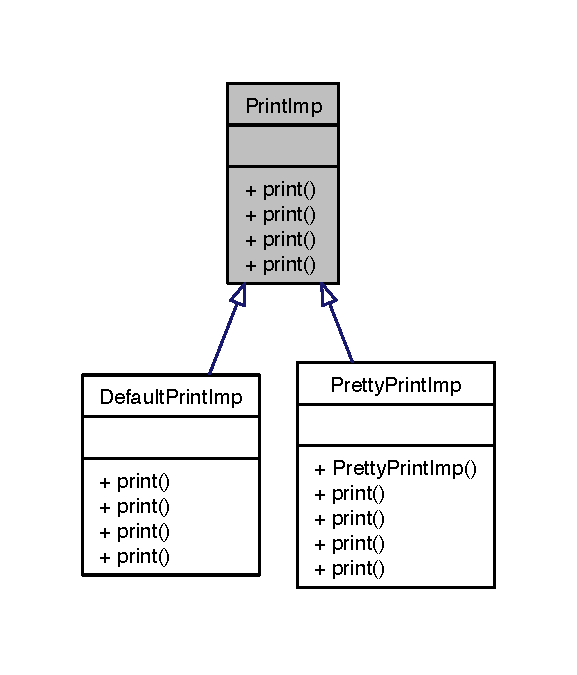
\includegraphics[width=277pt]{class_print_imp__inherit__graph}
\end{center}
\end{figure}
\subsection*{Public Member Functions}
\begin{DoxyCompactItemize}
\item 
\hypertarget{class_print_imp_a53a04c6deaa6f9203540d53d7cbaf19e}{virtual void {\bfseries print} (ostream \&, \hyperlink{class_json_value}{Json\-Value} $\ast$, int) const =0}\label{class_print_imp_a53a04c6deaa6f9203540d53d7cbaf19e}

\item 
\hypertarget{class_print_imp_a9788d3c8dd520f5fe568927baf85ca93}{virtual void {\bfseries print} (ostream \&, \hyperlink{class_pair}{Pair} $\ast$, int) const =0}\label{class_print_imp_a9788d3c8dd520f5fe568927baf85ca93}

\item 
\hypertarget{class_print_imp_a3df81c573b213d7836d4ba0a34694625}{virtual void {\bfseries print} (ostream \&, \hyperlink{class_json_object}{Json\-Object} $\ast$, int) const =0}\label{class_print_imp_a3df81c573b213d7836d4ba0a34694625}

\item 
\hypertarget{class_print_imp_ab56f3203d139681a195f8e86ee001acc}{virtual void {\bfseries print} (ostream \&, \hyperlink{class_json_array}{Json\-Array} $\ast$, int) const =0}\label{class_print_imp_ab56f3203d139681a195f8e86ee001acc}

\end{DoxyCompactItemize}


The documentation for this class was generated from the following file\-:\begin{DoxyCompactItemize}
\item 
Print\-Imp.\-h\end{DoxyCompactItemize}

\hypertarget{structyy__buffer__state}{\section{yy\-\_\-buffer\-\_\-state Struct Reference}
\label{structyy__buffer__state}\index{yy\-\_\-buffer\-\_\-state@{yy\-\_\-buffer\-\_\-state}}
}
\subsection*{Public Attributes}
\begin{DoxyCompactItemize}
\item 
\hypertarget{structyy__buffer__state_a4843d1422e3276b636d475a3095bd948}{F\-I\-L\-E $\ast$ {\bfseries yy\-\_\-input\-\_\-file}}\label{structyy__buffer__state_a4843d1422e3276b636d475a3095bd948}

\item 
\hypertarget{structyy__buffer__state_ad7b8df8d8a4688e57b0b8d3ca75adc85}{char $\ast$ {\bfseries yy\-\_\-ch\-\_\-buf}}\label{structyy__buffer__state_ad7b8df8d8a4688e57b0b8d3ca75adc85}

\item 
\hypertarget{structyy__buffer__state_a58aa927f098b99d99e75da80f9b681ef}{char $\ast$ {\bfseries yy\-\_\-buf\-\_\-pos}}\label{structyy__buffer__state_a58aa927f098b99d99e75da80f9b681ef}

\item 
\hypertarget{structyy__buffer__state_a48302f5f3477a9c78bbddf56d356ef54}{yy\-\_\-size\-\_\-t {\bfseries yy\-\_\-buf\-\_\-size}}\label{structyy__buffer__state_a48302f5f3477a9c78bbddf56d356ef54}

\item 
\hypertarget{structyy__buffer__state_a06406208824817acfec2183b79080945}{int {\bfseries yy\-\_\-n\-\_\-chars}}\label{structyy__buffer__state_a06406208824817acfec2183b79080945}

\item 
\hypertarget{structyy__buffer__state_a80ce2431c70dc4f89ced487f18449465}{int {\bfseries yy\-\_\-is\-\_\-our\-\_\-buffer}}\label{structyy__buffer__state_a80ce2431c70dc4f89ced487f18449465}

\item 
\hypertarget{structyy__buffer__state_abf5c70eea75581b58c0ee7bd31b14490}{int {\bfseries yy\-\_\-is\-\_\-interactive}}\label{structyy__buffer__state_abf5c70eea75581b58c0ee7bd31b14490}

\item 
\hypertarget{structyy__buffer__state_a9d60c60af6e1a6f69de16871fd64f85f}{int {\bfseries yy\-\_\-at\-\_\-bol}}\label{structyy__buffer__state_a9d60c60af6e1a6f69de16871fd64f85f}

\item 
\hypertarget{structyy__buffer__state_a63d2afbb1d79a3fc63df9e12626f827d}{int {\bfseries yy\-\_\-fill\-\_\-buffer}}\label{structyy__buffer__state_a63d2afbb1d79a3fc63df9e12626f827d}

\item 
\hypertarget{structyy__buffer__state_a70fd925d37a2f0454fbd0def675d106c}{int {\bfseries yy\-\_\-buffer\-\_\-status}}\label{structyy__buffer__state_a70fd925d37a2f0454fbd0def675d106c}

\end{DoxyCompactItemize}


The documentation for this struct was generated from the following file\-:\begin{DoxyCompactItemize}
\item 
lex.\-yy.\-c\end{DoxyCompactItemize}

\hypertarget{unionyyalloc}{\section{yyalloc Union Reference}
\label{unionyyalloc}\index{yyalloc@{yyalloc}}
}
\subsection*{Public Attributes}
\begin{DoxyCompactItemize}
\item 
\hypertarget{unionyyalloc_a4800e0520a89a4789afa7b5d82197e65}{yytype\-\_\-int16 {\bfseries yyss\-\_\-alloc}}\label{unionyyalloc_a4800e0520a89a4789afa7b5d82197e65}

\item 
\hypertarget{unionyyalloc_a9326f4fdc6f737a929444427836d8928}{Y\-Y\-S\-T\-Y\-P\-E {\bfseries yyvs\-\_\-alloc}}\label{unionyyalloc_a9326f4fdc6f737a929444427836d8928}

\end{DoxyCompactItemize}


The documentation for this union was generated from the following file\-:\begin{DoxyCompactItemize}
\item 
Json\-Parser.\-tab.\-c\end{DoxyCompactItemize}

\printindex
\end{document}
